\chapter{Cloud entrainment and mixing}
Another application of the current computing framework is the numerical study 
of turbulent entrainment and mixing processes at the boundary of a cloud. During the entrainment and mixing process, large eddies driven by the convective circulation engulf large volumes of environmental air deep into the cloud core. As turbulent mixing develops, these volumes are stretched and compressed into thinner filaments until the Kolmogorov scale is reached, where final homogenization occurs through the molecular diffusion process \cite{Burnet2007Observational}. Through entrainment and mixing with environment, the cloud water is diluted and transported by turbulence. In the previous bulk cloud models \cite{Grabowski1990Monotone}, the thermodynamic grid-averaged equations are used to describe the potential temperature, water vapor and cloud water mixing ratios. These model distinguish the evaporation and condensation scenarios according to the grid-averaged thermodynamic fields, and artificially adjust the grid box back to saturation as long as there is enough cloud water in the case of evaporation. This adjustment is based on the assumption that the vapor field in the subgrid cell is uniformly distributed during one time step. However, when the subgrid-scale structures of the thermodynamic fields exist, it is possible that the grid-averaged fields imply conditions below saturation and some cloud water does exist. Such conditions can occur, for instance, a part of the box is saturated and contains some cloud water, and the other part remains unsaturated and cloud-free \cite{Grabowski2007}. In many literatures\cite{Baker1980, Burnet2007Observational, Lehmann2009}, two extreme cases are usually used to describe the mixing processes: extremely homogeneous mixing and extremely inhomogeneous mixing. In the extremely homogeneous case, the mixing process is so fast that all the cloud droplets stay in the same environment, and yet in the extremely inhomogeneous scenario, a part of the droplets completely disappear before others begin to evaporate. In consequence, the homogeneous mixing only changes the averaged droplets size before completely evaporation happens, while the inhomogeneous mixing remains the mean droplets size with a decreasing number density.

The entrainment and mixing process is important for the evolution of a cloud, but until now it was poorly understood that whether the reduction of liquid water content during entrainment was through the reduction of only the droplet size (extremely homogeneous mixing), or only the number of droplets (extremely inhomogeneous mixing), or both the number and size (inhomogeneous mixing). These situations can be quantified by comparing two time scales: the turbulent homogenization time scale and thermodynamic time scale associated with the evaporation process. In the extreme cases, one time scale will dominate the other, otherwise the two scales are comparable. Recently, it has been demonstrated that different mixing scenarios can occur and change during one single cloud evolution (\cite{Andrejczuk2009,Burnet2007Observational,Lehmann2009}) and therefore it becomes more and more important to have a reasonable and accurate estimation of the mixing scenario for a subgrid model. \cite{Jarecka2013}, utilized the DNS results from \cite{Andrejczuk2004, Andrejczuk2006, Andrejczuk2009}  to estimate the mixing scenario with a parameter $\alpha$ and merged the $\lambda$-$\beta$ subgrid scheme (\cite{Jarecka2009}) with the double-moment LES model(\cite{Morrison2008}). \cite{Lu2013}, proposed the transition scale number to measure the occurrence probability of homogeneous or inhomogeneous entrainment-mixing process (homogeneous mixing degree). Both the cloud observations and numerical simulations imply a positive relationship between the transition scale number and the homogeneous mixing degree. In spite of many progresses in the study of cloud microphysics, to capture the details of turbulent transportation and dilution of cloud water remains a challenge for representing clouds in coarse-resolution climate model.

In this section, we describe a new particle-resolved three dimensional direct numerical simulation (DNS) model that combines Lagrangian droplet tracking with the Eulerian field representation. The new model consists of the turbulence environment, scalar fields and particle system, and thus can be easily built under the computational framework proposed in this paper.

\section{Model Description}
Similar to most previous DNS, our new DNS is based on the incompressible
Boussinesq fluid system \cite{Andrejczuk2004}. Briefly, the temperature $T$ and vapor
mixing ratio $q_v$ are described by the following equations \cite{Kumar2012Cloud}:

\begin{equation}
\partial_{t}T+(\mathbf{u}\cdot\nabla)T=\frac{L_{h}}{c_{p}}C_{d}+\mu_{T}\nabla^{2}T\label{eq:Temp}
\end{equation}

\begin{equation}
\partial_{t}q_{v}+(\mathbf{u}\cdot\nabla)q_{v}=-C_{d}+\mu_{v}\nabla^{2}q_{v}\label{eq:Vapor}
\end{equation}

where $L_{h}$ is the latent heat of water vapor condensation,
$c_{p}$ is the specific heat at constant pressure, $\mu_{T}=\mu_{v}$ are
the molecular diffusivity for temperature and water vapor, respectively
and assumes to be equal. The condensation rate $C_{d}$ denotes the rate of exchange between liquid and vapor, and is described by:

\begin{subequations}

\begin{equation}
C_{d}(\mathbf{X},t)=\frac{d(m_{l}(\mathbf{X},t))}{m_{a}dt}=\frac{4\pi\rho_{l}K}{\rho_{0}a^{3}}\Sigma_{i=1}^{n}S(\mathbf{X}_{i},t)R_{i}(t)\label{eq:CondRate}
\end{equation}


where $K$ is a function of temperature and pressure given by:

\begin{equation}
K=1/[(\frac{L_{h}}{R_{v}T}-1)\frac{L_{h}\rho_{l}}{C_{T}T}+\frac{\rho_{l}R_{v}T}{De_{s}(T)}]\label{eq:CondCoeff}
\end{equation}


where $R_{v}$ is the individual gas constant, 
$C_{T}$ is the coefficient of thermal conductivity, $e_{s}(T)$ is
the saturation vapor pressure. The supersaturation $S(X,t)$ is calculated
directly from the water vapor mixing ratio and temperature from the following
equation

\begin{equation}
S(\mathbf{X},t)=\frac{q_{v}(\mathbf{X},t)}{q_{v,s}(\mathbf{X},t)}-1\label{eq:Supersat}
\end{equation}

\end{subequations}

where $q_{v,s}$ is the corresponding saturated water vapor mixing ratio. The droplets
will grow or shrink depending on the sign of supersaturation $S$.

The liquid water mixing ratio is given by
\begin{equation}
q_{c}(\mathbf{X},t)=\frac{4\pi\rho_{l}}{3\rho_{0}a^{3}}\sum_{i=1}^{n}R_{i}^{3}(t)\label{eq:cloud_water}
\end{equation}


where $a$ is the size of a grid cell, $n$ is the number of droplets
in the grid cell; $\rho_{l}$ and $\rho_{0}$ are the densities of water
and air. $R_{i}(t)$ is the radius of the $i$-th droplet.

The dynamical field is given by
\begin{subequations}

\begin{equation}
\partial_{t}\mathbf{u}+(\mathbf{u}\cdot\nabla)\mathbf{u}=-\frac{1}{\rho_{0}}\nabla p+\nu\nabla^2 \mathbf{u}+\mathbf{f}_b + \mathbf{f}_e\label{eq:NS1}
\end{equation}


\begin{equation}
\nabla\cdot \mathbf{u}=0\label{eq:NS2}
\end{equation}

\end{subequations}

where $\nu$ is the kinetic viscosity, $\rho_{0}$ is the density of
dry air, $\mathbf{u}$ is the velocity field, $p$ is the pressure field. Here $\mathbf{f}_b$ is the force immitating the buoyancy effects:
\begin{equation}
\mathbf{f}_b= 
-\mathbf{g}[\frac{T-T_{0}}{T_0}+0.608(q_{v}-q_{v0})-q_{c}]
\label{eq:source_term}
\end{equation}
where $\mathbf{g}$ is the gravity, $T$ and $q_{v}$ are temperature
and vapor mixing ratio field respectively with the subscript ``$0$''
denoting the reference value. $\mathbf{f}_e$ is the artificial external force defined in the Fourier space.

To describe the motion and condensation(or evaporation) of cloud droplets, we use

\begin{equation}
R(t)\frac{R(t)}{dt}=K\cdot S(\mathbf{X},t)\label{eq:Radius}
\end{equation}


\begin{equation}
\frac{d\mathbf{X}(t)}{dt}=\mathbf{V}(t)\label{eq:Coords}
\end{equation}


\begin{equation}
\frac{d\mathbf{V}(t)}{dt}=\frac{1}{\tau_{p}}[\mathbf{u}(\mathbf{X},t)-\mathbf{V}(t)]+\mathbf{g}\label{eq:Velocity}
\end{equation}

Here $R(t)$ is the radius, $\mathbf{X}(t)$ is the position coordinate and
$\mathbf{V}(t)$ is the droplet velocity, $\mathbf{g}$ is the gravitational
constant. $\tau_{p}=2\rho_{l}R^{2}/(9\rho_{0}\nu)$ is the finite particle
response time. The particle response time measures the droplet inertial
effects; when $\tau_{p}$ is set to be zero, equation (\ref{eq:Velocity})
becomes $\mathbf{V}(t)=\mathbf{u}(\mathbf{X},t)$, which implies that the
droplets will exactly follows the turbulent flows. The last term in equation
(\ref{eq:Velocity}) is the sedimentation term that accounts for the effect of
gravity on droplets motion. Equation (\ref{eq:Velocity}) is appropriate if the
Reynolds number based on the relative velocity between the particle and fluid
is significantly less than one \cite{Eaton1994}. The particle diameter is also
assumed to be smaller than the Kolmogorov microscale $\eta$, the smallest
length scales of the turbulent flow field. During condensation, direct
interactions between droplets are negligible because their sizes are too small
comparing with the average distance between two droplets.

The dynamic equations \Eq{eq:NS1} and \Eq{eq:NS2} are solved following the
fraction-step algorithm \cite{Brown2001Accurate}. The thermodynamic fields
\Eq{eq:Temp}, \Eq{eq:Vapor} are solved with semi-implicit method coupling with
fifth-order WENO scheme for the discretization of the hyperbolic term. The use
of WENO scheme here is critical since it can well handle the numerical
overshoots as well as keep the high order of the overall accuracy. To simplify
the implementation, we adopt the external package PETSc \cite{petsc_cite} as
the parallel linear solver and HYPRE \cite{hypre_cite} as the high performance
preconditioner. These two packages are widely used in the community of
computational fluid dynamics and has a good parallel scaling in both Linux
cluster and supercomputer.The Droplets position (\Eq{eq:Coords}) and motion
(\Eq{eq:Velocity}) are solved by implicit Euler method in consideration of
efficiency and stability. The time step size is adaptive to satisfy the
Courant-–Friedrichs-–Lewy (CFL) condition. Parallel computing techniques are
implemented with MPI library to increase the computational speed.

\section{Turbulence initialization and external forcing}
Since the DNS is performed in a small-scale turbulence environment, it is necessary to generate and maintain a physical turbulence field before injecting the particles into it. Many literatures \cite{Eswaran1988} have demonstrated that the small-scale behavior in turbulent flows tends to be characterized by statistical homogeneity, isotropy and universality. Because of the universality we can hope to understand small-scale behavior by studying the simplest turbulent flows: homogeneous, isotropic turbulence. The two most frequently studied types of isotropic turbulence are freely decaying, and forced statistically stationary turbulence, which are both studied in this dissertations. The decaying turbulence can be easily obtained by providing a solenoidal isotropic initial velocity field with random phases and prescribed energy spectrum, and then directly solve the Navier-Stokes equation to evolve the turbulence. In addition to the initial condition, the forced turbulence further requires a method to artificially force the low-wavenumber modes, so as to supply the energy dissipated by viscous effects. The energy-containing motions are, therefore, unnatural and are not governed by the Navier-Stokes equations. However, insofar as the small-scale motions are universal, useful information about them can be extracted provided that there is wide separation between the largest and smallest scales. The initialization and external forcing method for homogeneous, isotropic turbulence are introduced below. 

Similar to Rogallo's procedure, the initial velocity field is constructed in Fourier space satisfying continuity, isotropy, and having a given energy spectrum. Given the coordinates in three-dimensional Fourier space $\vect{k} = \{k_1, k_2, k_3\}$ and energy spectrum $E(k)$, the Fourier transformation $\hat{\vect{u}}$ of the velocity field is determined by:
\begin{equation}
\hat{\vect{u}} = \left\{\frac{\alpha kk_2 + \beta k_1k_3}{k(k_1^2 + k_2^2)^{1/2}},
\frac{\beta k_2k_3 - \alpha k k_1}{k(k_1^2 + k_2^2)^{1/2}}, 
- \frac{\beta (k_1^2 + k_2^2)^{1/2}}{k}\right\}
\end{equation}
where $k = (k_1^2 + k_2^2 + k_3^2)^{1/2}$. The coefficients $\alpha$ and $\beta$ are 
\begin{equation}
\alpha = (\frac{E(k)}{4\pi k^2})^{1/2}e^{i\theta_1}\cos{\phi},\quad
\beta = (\frac{E(k)}{4\pi k^2})^{1/2}e^{i\theta_2}\sin{\phi}
\end{equation}
where $\theta_1$, $\theta_2$, and $\phi$ are uniformly distributed random numbers on the interval $(0, 2\pi)$. It can be verified that $\hat{\vect{u}}$ satisfies the continuity condition $\hat{\vect{u}}\cdot\vect{k} = 0$
The energy function is defined as:
\begin{equation}
E(k) = \frac{16}{\sqrt{\pi/2}}\frac{u^2_{rms}k^4}{k_0^5}\exp(-\frac{2k^2}{k_0^2})
\end{equation}
where $u_{rms}$ is the initial root-mean-square (r.m.s) velocity, and $k_0$ is the wavenumber at which the maximum of $E(k)$ occurs. The parameters $u_0$ and $k_0$ determine
the exact power spectral shape. Different from the commonly used Kolmogorov
spectrum, this function enforces the kinetic energy be concentrated in a
relatively narrow band at the initial time, so as to not affect the turbulence
behavior in larger wave number space. As turbulence evolves, the spectrum will
quickly spread to the inertial range and dissipation range according to the
Navier-Stokes equation. \Fig{fig:eng_spr} illustrates the energy spectrum with
different parameters. The parameters for most cases in this paper are $u_0 =
0.35m/s$ and $k_0 = |(1,1,2)| \approx 2.4$, which allows one to generate an
initial turbulence field with reasonable Reynolds number and narrow energy band
in large wave length.

\begin{figure}[!htbp]\centering
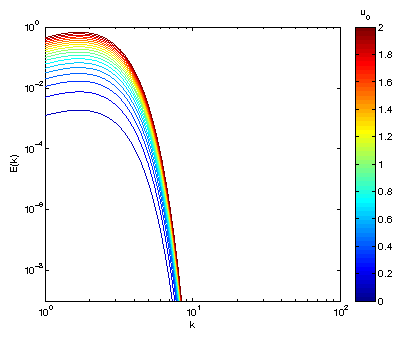
\includegraphics[width=0.48\textwidth]{Figures/eng_spr_u}
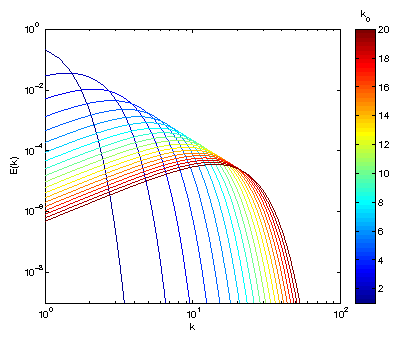
\includegraphics[width=0.48\textwidth]{Figures/eng_spr_k}
\caption{Initial energy spectrum with different parameters: left figure shows the energy spectrum with fixed $k_0 = 2.4$ while varing $u_0$ from $0m/s$ to $2m/s$, right figure shows the one with fixed $u_0 = 0.35m/s$ and varing $k$ from $1$ to $20$.\label{fig:eng_spr}}
\end{figure}

As for the external volume force, several solutions have been proposed in the literature, representing two main approaches. The first is to construct the force in Fourier space to keep a constant energy injection rate, and thus this method requires knowledge of Fourier-transformed velocities. In \cite{Ghosal1995Dynamic, Carati1995Representation}, the authors applied a force to the wavenumbers in the chosen shell, and guarantee a constant energy injection rate. The Ghosal's approach can be simply formulated in the Fourier space: 
\begin{equation}
\mathbf{f}_e(\mathbf{k},t) = \epsilon_{in}\frac{\mathbf{u}(\mathbf{k},t)}
{\sum_{\mathbf{k}_f\in \kappa}|\mathbf{u}(\mathbf{k}_f,t)|^2}
\sigma_{\mathbf{k},\mathbf{k}_f}
\end{equation}
where $\mathbf{u}(\mathbf{k},t)$ is the Fourier-transformed velocity function, $\mathbf{k}_f$ is chosen from a subset of the wavenumber space $\kappa$ containing a few wavevectors, for example $(1,1,2)$ plus all permutations with respect to components and sign, $\epsilon_{in}$ is a constant input energy rate. $\delta_{k,k_f}$ is a delta function. Therefore, statistics stationary homogeneous turbulence can be obtained in DNS by forcing the low-wavenumber modes. There still exist many other approaches based on the Fourier transformation. For example, Sullivan and Chasnov attempted to maintaining constant kinetic energy in the lowest wavenumbers \cite{Sullivan1994Deterministic, Chasnov1991Simulation}. Eswaran and Pope in \cite{Eswaran1988} utilized a stochastic process to determine external forcing scheme. 

The second group is to evaluate the external force in physical space. This approach is attractive for applications since it does not require transformation to Fourier space and is easily integrated into physical-space numerical codes. Lundgren proposed a forcing function which is directly proportional to the velocity \cite{Lundgren2003Linearly}. Rosales studied the properties of this linear forcing scheme for isotropic turbulence, and showed the linearly forced system converges to a stationary state that does not depend on the spectral shape of the initial condition \cite{Rosales2005Linear}. The Lundgren's linear forcing scheme is determined with the following equation:
\begin{equation}
\vect{f}(\vect{x}, t) = \frac{\epsilon_{in}}{3u_{rms}^2}\vect{u}
\end{equation}
During the simulation, the root-mean-square velocity $u_{rms}$ is recalculated every time step while the energy injection rate $\epsilon_{in}$ is kept equal to a constant.
The cross section of the initial and stationary vorticity field is displayed in \Fig{fig:vort}.

\begin{figure}[!htbp]\centering
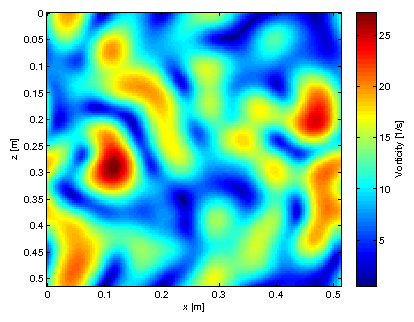
\includegraphics[width=0.45\textwidth]{Figures/vortex-0}
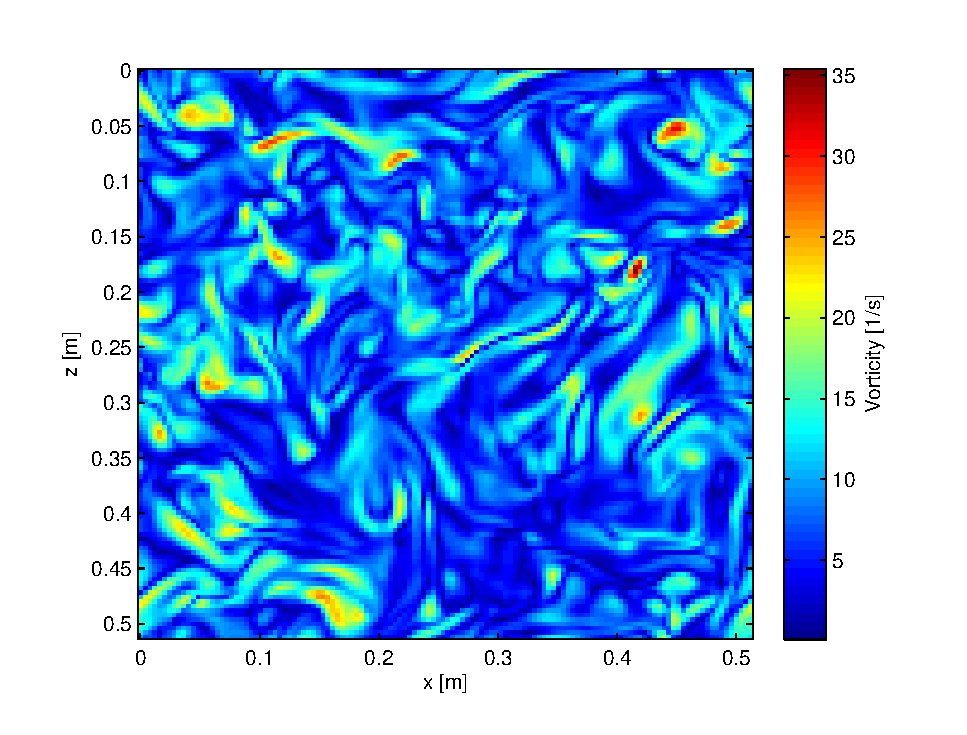
\includegraphics[width=0.45\textwidth]{Figures/vortex-1}

\caption{initial and final vorticity field ($1/s$) in x-z cross-sectional
plane for forced cases\label{fig:vort}}
\end{figure}

\section{Parallelism}
The numerical experiments for DNS of cloud entrainment mixing are carried out on the Linux cluster ``FASTER", named after the FASTER (Fast-Physics-System-Testbed and Research) project. The parallelization of this application involves three components: computation of fluid dynamics, computation of particles and runtime data analysis. The parallelization for the computation of fluid dynamics is done through domain decomposition and buffer extension. The computational domain is first uniformly divided into several partitions, and each partition has a buffer in each direction storing the information of its neighbor cells. The buffer is then updated every time step to provide the boundary information for the finite difference method. A typical $4\times 4\times 4$ partition of the computational domain is displayed in \Fig{fig:droplets_parallel}. 

\begin{figure}[!htbp] \centering
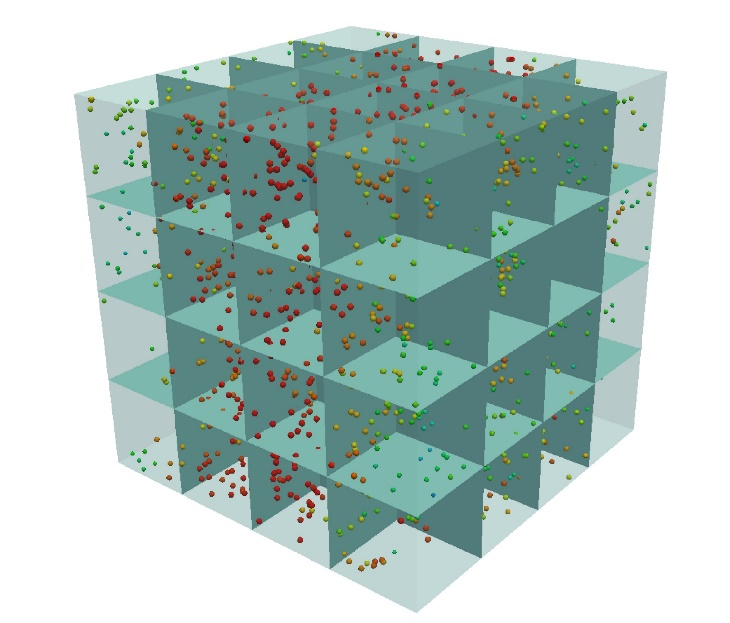
\includegraphics[width=0.7\textwidth]{Figures/droplets_parallel.jpg}
\caption{$4\times 4\times 4$ partitions of computational domain for the simulation of 
cloud droplets\label{fig:droplets_parallel}} 
\end{figure}

The computation of the particles is parallelized using a hybrid computing technique. After each time step, the particles with zero radius or exceeding the limits of the local domain are removed from the current partition or sent to its neighbors. The computation can be further accelerated using Open-MP or GPU technique within one time step. The combination of using MPI between computing nodes and shared memory computing inside a node results in a hybrid computing technique, which has become the mainstream of high performance computing.
In addition, the runtime data analysis also needs parallelization. For example, a parallel algorithm is required to calculate the mean and standard deviation of the droplets radius, temperature field, vapor mixing ratio field and velocity field. The calculation is first carried out in each processor by itself, and then aggregated to the answer using MPI reduce subroutine. However, since the size of the numbers $n$ is too large ($n = O(10^7)$ for cloud droplets and $n = O(10^6)$ for fields), simply summing a sequence of finite precision floating point numbers may accumulate the numerical error. To overcome this, we have applied the Kahan summation algorithm \cite{Kahan1965Pracniques}, in which the worst-case error bound is independent of $n$. Therefore, a large number of values can be summed with an error that only depends on the floating-point precision. 

Next chapter gives a detailed description of the numerical experiments and results. The data processing and analysis will also be presented.
\newpage{}
